\documentclass[11pt,a4paper]{article}

\usepackage[margin=1in, paperwidth=8.3in, paperheight=11.7in]{geometry}
\usepackage{amsfonts}
\usepackage{amsmath}
\usepackage{amssymb}
\usepackage{array}
\usepackage{enumerate}
\usepackage{enumitem}
\usepackage{fancyhdr}
\usepackage{graphicx}
\usepackage{tikz}
\usepackage{changepage} 

\begin{document}

\pagestyle{fancy}
\setlength\parindent{0pt}
\allowdisplaybreaks

\renewcommand{\headrulewidth}{0pt}

%New column type
\newcolumntype{L}[1]{>{\arraybackslash}m{#1cm}}

% Cover page title
\title{Image Processing and Computer Vision - Notes}
\author{Dom Hutchinson}
\date{\today}
\maketitle

% Header
\fancyhead[L]{Dom Hutchinson}
\fancyhead[C]{Image Processing and Computer Vision - Notes}
\fancyhead[R]{\today}

% Counters
\newcounter{definition}[section]
\newcounter{example}[section]
\newcounter{notation}[section]
\newcounter{proposition}[section]
\newcounter{remark}[section]
\newcounter{theorem}[section]

% commands
\newcommand{\dotprod}[0]{\boldsymbol{\cdot}}
\newcommand{\cosech}[0]{\mathrm{cosech}\ }
\newcommand{\cosec}[0]{\mathrm{cosec}\ }
\newcommand{\sech}[0]{\mathrm{sech}\ }
\newcommand{\blocks}[0]{\mathbb{B}}
\newcommand{\nats}[0]{\mathbb{N}}
\newcommand{\real}[0]{\mathbb{R}}
\newcommand{\integers}[0]{\mathbb{Z}}
\newcommand{\nb}[0]{\textit{N.B.} }
\newcommand{\eg}[0]{\textit{e.g.} }

\newcommand{\definition}[1]{\stepcounter{definition} \textbf{Definition \arabic{section}.\arabic{definition}\ - }\textit{#1}\\}
\newcommand{\example}[1]{\stepcounter{example} \textbf{Example \arabic{section}.\arabic{example}\ - }\textit{#1}\\}
\newcommand{\notation}[1]{\stepcounter{notation} \textbf{Notation \arabic{section}.\arabic{notation}\ - }\textit{#1}\\}
\newcommand{\proposition}[1]{\stepcounter{proposition} \textbf{Proposition \arabic{section}.\arabic{proposition}\ - }\textit{#1}\\}
\newcommand{\remark}[1]{\stepcounter{remark} \textbf{Remark \arabic{section}.\arabic{remark}\ - }\textit{#1}\\}
\newcommand{\theorem}[1]{\stepcounter{theorem} \textbf{Theorem \arabic{section}.\arabic{theorem}\ - }\textit{#1}\\}

\tableofcontents

% Start of content
\newpage

\section{Image Acquistion}

\proposition{Common Challenges with Image Acquistion}
Below are some common challeges that are faced/produced by image acquistion\\
\begin{tabular}{|l|L{12}|}
\hline
Viewpoint Variation&Several images may be taken of the same object but will vary the angle\\
Illumination&Images may be taken in low/high light\\
Occlusion&Object may be partly obscured\\
Scale&Objects may look vary different when placed next to other objects due to their relative scale\\
Deformation&Objects may have slight variations on the perfect form\\
Background Clutter&Lots happening behind an object may work to obscure it\\
Object Intra-Class Variation&Some objects in the same class can vary a lot in shape (\eg chairs)\\
Local Ambiguity&Certain regions of an image can be missinturpred without the rest of the scene being accounted for\\
World Behind the Image&Depth may need to be accounted for to make sense of an image.\\
\hline
\end{tabular}\\

\definition{Dirac Delta-Function, $\delta$}
The \textit{Dirac Delta-Function} is used to map continuous distributions to discrete distributions by sampling at particular intervals. Intuitively
$$\delta(t)=\begin{cases}1&, t=0\\0&, t\neq0\end{cases}\implies\delta(t-\alpha)=\begin{cases}1&, t=\alpha\\0&, t\neq\alpha\end{cases}$$

\definition{Sifting Property}
We can apply the \textit{Dirac Delta-Function} to a function to sample a particular value
$$\int_{-\infty}^\infty f(t)\delta(t)dt=f(0)\implies\int_{-\infty}^\infty f(t)\delta(t-\alpha)dt=f(\alpha)$$
This can be applied to 2D objects (such as images) as
$$\int_{-\infty}^\infty f(a,b)\delta(a-x,b-y)dadb=f(x,y)$$

\definition{Point Spread-Function}
A \textit{Point Spread-Function} is applied after sampling an image. It takes the value of a pixel \& transforms pixels around it using this value in some way.\\
\eg\raisebox{-0.5\height}{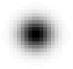
\includegraphics[scale=1]{img/psf.png}}

\section{Image Representation}

\definition{Colour Space}
\textit{Colour Space} are different techniques for representing colours. These are generally made up of 3D vectors.\\
\begin{tabular}{|l|L{13}|}
\hline
Colour Space&Vector Description\\
\hline
RGB&(Red $\in[0,255]$,Green $\in[0,255]$,Blue $\in[0,255]$)\\
HSI&(Hue $\in[0,360)$,Saturation $\in[0,1]$,Intensity $\in[0,1]$)\newline Hue gives the colour in degrees\\
YUV&(Brightness $\in[0,255]$,Blue Projection $\in[0,255]$,Red Projection $\in[0,255]$)\\
La*b*&(Luminance $\in[0,100]$, Red/Green $\in\{-a,+b\}$, Blue/Yellow $\in\{+b,-b\}$\\
\hline
\end{tabular}\\

\remark{Representing Video}
To represent video each fixel is given a third parameter, $time$ so we now have
$$f(x,y,t)\mapsto(R,G,B)$$
or any other \textit{Colour Space}.\\

\definition{Quantisation}
\textit{Quantisation} is representing a continuous single channel function with discrete single channel function that groups the continuous values into a set number of levels.\\

\example{Quantisation}
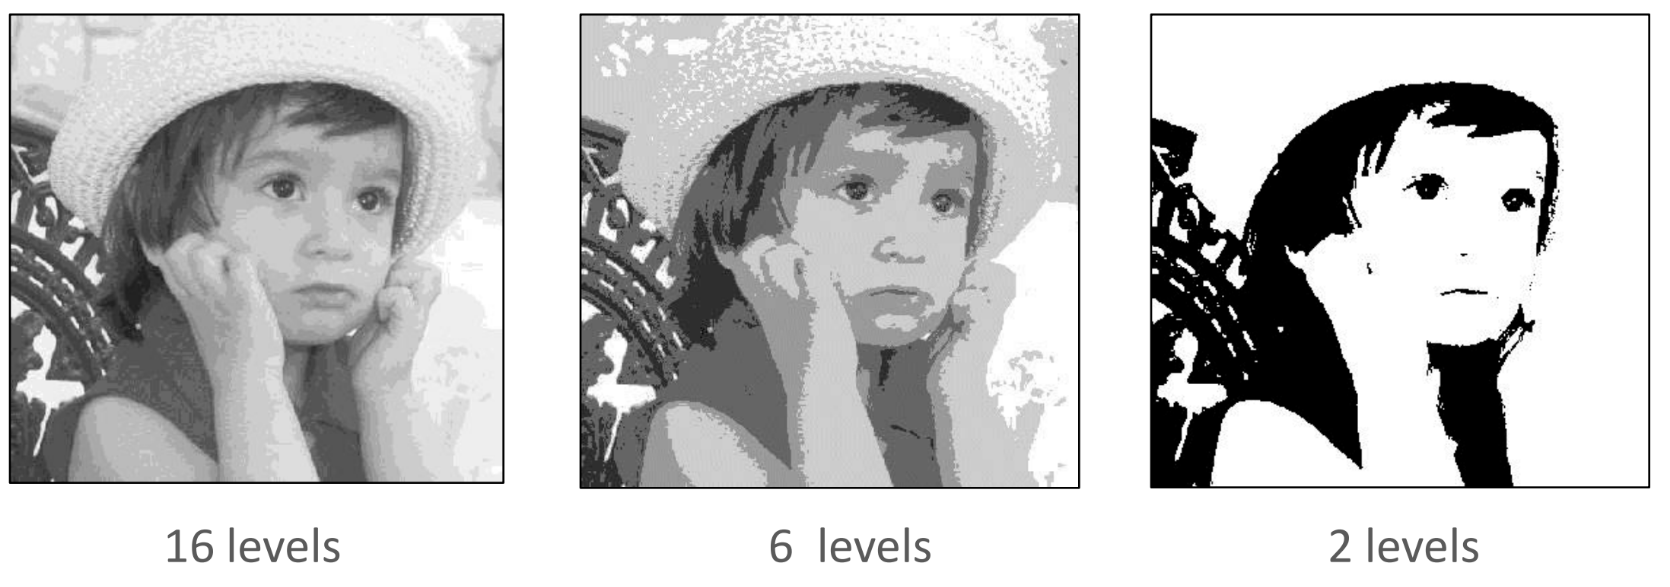
\includegraphics[scale=.3]{img/quantisation.png}

\definition{Aliasing}
\textit{Aliasing} is the result of sparse sampling since single pixels represent to large an area to get any detail out of it.\\

\example{Aliasing}
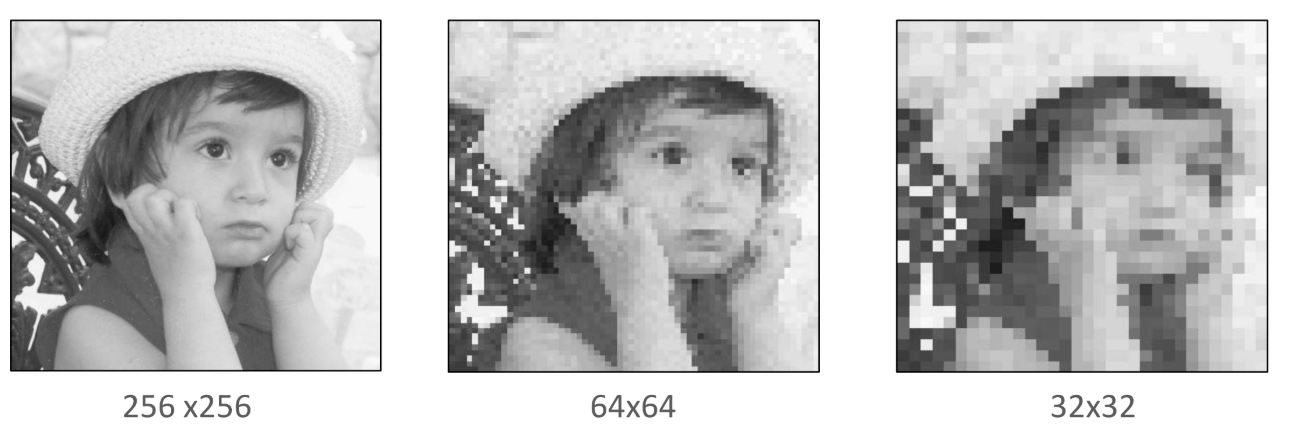
\includegraphics[scale=.4]{img/aliasing.png}

\definition{Anti-Aliasing}
\textit{Anti-Aliasing} is the process for avoiding \textit{Aliasing}. This can be achieved by using a sampling rate which is a critical limit defined by the \textit{Shannon-Nyquist Theorem}.\\

\theorem{Shannon-Nyquist Theorem}
An analogue signal with maximum frequency $x\text{Hz}$ may be completley reconstructed if regular samples are taken with frequency $2x\text{Hz}$.\\

\definition{Convolution}
\textit{Convolution} is an operation which takes two functions \& produces a third which describes how the shape of one of the two functions is changed by the other.\\
For functions $f\ \&\ g$
$$(f*g)(x):=\int_{-\infty}^\infty f(x-t)h(x)\partial t$$
\nb $*$ is the symbol for convolution.\\

\remark{Convolution in Image Representation}
Suppose you have a system, represented by kernel $g(x)$, \& an input signal, represented by $f(x)$. THen $f*g(x)$ describes the effect of the system on the input signal. The resulting image is called the \textit{Response of $f$ to the kernel $h$}.\\
%TODO what is a kernel

\proposition{2D Discrete Convolution}
Since images are represnted by discrete 2D functions $f:\nats\times\nats\to(\nats\times\nats\times\nats)$ it is pertinent to understand \textit{2D Discrete Convolution}.\\
$$h(x,y)=\sum_{i\in I}\sum_{j\in J}f(x-i,y-j)g(i,j)$$
Often the kernel, $g(x,y)$, has negative indices so the pixel being acted upto is equivalent to the middle pixel in the matrix representation of $g(x,y)$.\\
\nb A convolution whose kernel is symmetric on 180 degree rotation is called a \textit{Correlation}.

\example{2D Discrete Convolution}
Below is a representation of a grayscale image, $f(x,y)$, on the left \& a kernel $g(x,y)$ on the right.
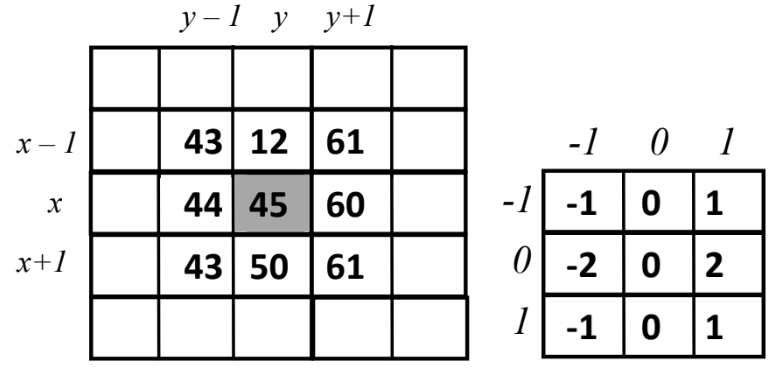
\includegraphics[scale=.3]{img/2dconvolution.png}\\
$(f*g)(x,y)=f(x+1,y+1)g(-1,-1)+f(x+1,y)g(0-1,0)+\dots+f(x-1,y-1)g(1,1)=-68$.\\

\remark{High/Loss Pass Filtering}
Kernels can be defined for specific desired effects on an image through convolution.\\
\begin{enumerate}[label=\roman*)]
\item An image can be made more fuzzy using a \textit{Low Pass Kernel}
$$\begin{pmatrix}1&1&1\\1&1&1\\1&1&1\end{pmatrix}$$
\item An image can be made sharper using a \textit{High Pass Kernel}
$$\begin{pmatrix}-1&-1&-1\\-1&8&-1\\-1&-1&-1\end{pmatrix}$$
\end{enumerate}


\end{document}